\documentclass[12pt, a4paper]{article}
\usepackage{../../../myconfig} % Gọi file cấu hình từ ngoài gốc vào

% ==========================================
% BẮT ĐẦU NỘI DUNG TÀI LIỆU
% ==========================================
\begin{document}

% Truyền 3 tham số: {Nhãn cam} {Chữ to chính giữa} {Chữ ở góc phải Header}
\titlebox{Chủ đề: định kì}{Đề kiểm tra định kì lần 6}{Đề định kì}

\textit{\textbf{Phần I: Thí sinh trả lời từ câu 1 đến câu 12, mỗi câu thí sinh chỉ chọn một phương án}}

\vspace{0.5cm}

% --- CÂU 1 ---
\questionLinesManual{0}{1}{Cho \((C \in \mathbb{R})\). Tính \(I = \displaystyle\int (x^2 + 3)x^2 dx\).}{%
    \begin{tasks}(2)
        \task \(I = \dfrac{x^5}{5} + x^3 + C\)
        \task \(I = \dfrac{x^5}{5} + x^3\)
        \task \(I = \left( \dfrac{x^3}{3} + 3x \right)\dfrac{x^3}{3} + C\)
        \task \(I = x^4 + 3x^2 + C\)
    \end{tasks}
}

% --- CÂU 2 ---
\questionLinesManual{0}{2}{Cho \((C \in \mathbb{R})\). Chọn khẳng định \textbf{sai} trong các khẳng định sau.}{%
    \begin{tasks}(2)
        \task \(\displaystyle\int e^x dx = e^x + C\)
        \task \(\displaystyle\int \sin x dx = -\cos x + C\)
        \task \(\displaystyle\int \dfrac{1}{x^2} dx = -\dfrac{1}{x} + C\) \((x \neq 0)\)
        \task \(\displaystyle\int a^x dx = a^x + C\)
    \end{tasks}
}

% --- CÂU 3 ---
\questionLinesManual{0}{3}{Tính tích phân \(L = \displaystyle\int_{0}^{\frac{\pi}{3}} (2\sin x + 1) dx\).}{%
    \begin{tasks}(4)
        \task \(L = \dfrac{\pi}{3} - 1\)
        \task \(L = \dfrac{\pi}{3} - 3\)
        \task \(L = 1 - \dfrac{\pi}{3}\)
        \task \(L = 1 + \dfrac{\pi}{3}\)
    \end{tasks}
}

% --- CÂU 4 ---
\questionLinesManual{0}{4}{Tính \(\displaystyle\int \sin\left( 2x + \dfrac{\pi}{2} \right) dx\).}{%
    \begin{tasks}(2)
        \task \(I = -\cos\left( 2x + \dfrac{\pi}{2} \right) + C\)
        \task \(I = 2\cos\left( 2x + \dfrac{\pi}{2} \right) + C\)
        \task \(I = -\dfrac{1}{2}\cos\left( 2x + \dfrac{\pi}{2} \right) + C\)
        \task \(I = \dfrac{1}{2}\cos\left( 2x + \dfrac{\pi}{2} \right) + C\)
    \end{tasks}
}

% --- CÂU 5 ---
\questionLinesManual{0}{5}{Cho hàm số \(f(x)\) liên tục trên đoạn \([a; b]\). Hãy chọn mệnh đề \textbf{sai}.}{%
    \begin{tasks}(2)
        \task \(\displaystyle\int_{a}^{b} f(x) dx = \int_{b}^{a} f(x) dx\)
        \task \(\displaystyle\int_{a}^{b} k dx = k(b - a), \forall k \in \mathbb{R}\)
        \task \(\displaystyle\int_{a}^{b} f(x) dx = -\int_{b}^{a} f(x) dx\)
        \task \(\displaystyle\int_{a}^{b} f(x) dx = \int_{a}^{c} f(x) dx + \int_{c}^{b} f(x) dx, c \in [a; b]\)
    \end{tasks}
}

% --- CÂU 6 ---
\questionLinesManual{0}{6}{Biết \(F(x)\) là nguyên hàm của hàm \(f(x) = \dfrac{1}{x-1}\) và \(F(2) = 1\). Tính \(F(3)\).}{%
    \begin{tasks}(4)
        \task \(F(3) = \ln 2\)
        \task \(F(3) = \ln 2 + 1\)
        \task \(F(3) = \ln \dfrac{3}{2}\)
        \task \(F(3) = \dfrac{1}{2}\)
    \end{tasks}
}

% --- CÂU 7 ---
\questionLinesManual{0}{7}{Cho \(f(x)\) là hàm số liên tục trên đoạn \([a; b]\). Giả sử \(F(x)\) là một nguyên hàm của hàm \(f(x)\) trên đoạn \([a; b]\). Khẳng định nào sau đây là khẳng định \textbf{đúng}?}{%
    \begin{tasks}(2)
        \task \(\displaystyle\int_{a}^{b} f(x) dx = F(b) - F(a) + C\)
        \task \(\displaystyle\int_{a}^{b} f(x) dx = F(a) - F(b)\)
        \task \(\displaystyle\int_{a}^{b} f(x) dx = F(b) - F(a)\)
        \task \(\displaystyle\int_{a}^{b} f(x) dx = F(a) - F(b) + C\)
    \end{tasks}
}

% --- CÂU 8 ---
\questionLinesManual{0}{8}{Tích phân \(\displaystyle\int_{0}^{1} \dfrac{1}{x^2 - x - 12} dx = \dfrac{2}{a}\ln\dfrac{b}{c}\) thì \(a + b + c\) bằng:}{%
    \begin{tasks}(4)
        \task 7
        \task 14
        \task 10
        \task \(\dfrac{31}{4}\)
    \end{tasks}
}

% --- CÂU 9 ---
\questionLinesManual{0}{9}{Diện tích hình phẳng được giới hạn bởi đồ thị hàm số \(y = x^3\), trục hoành và hai đường thẳng \(x = -1\), \(x = -2\).}{%
    \begin{tasks}(4)
        \task 17
        \task \(\dfrac{15}{4}\)
        \task \(\dfrac{17}{4}\)
        \task 4
    \end{tasks}
}

% --- CÂU 10 ---
\questionLinesManual{0}{10}{Cho hàm số \(f(x) = x(x-2)(x-4)\). Diện tích hình phẳng giới hạn bởi đồ thị hàm số và trục \(Ox\) là:}{%
    \begin{tasks}(2)
        \task \(\displaystyle\int_{0}^{4} f(x) dx\)
        \task \(\left| \displaystyle\int_{0}^{4} f(x) dx \right|\)
        \task \(\displaystyle\int_{0}^{2} f(x) dx - \int_{2}^{4} f(x) dx\)
        \task \(\displaystyle\int_{0}^{2} f(x) dx + \int_{2}^{4} f(x) dx\)
    \end{tasks}
}

% --- CÂU 11 ---
\questionLinesManual{0}{11}{Diện tích hình phẳng được giới hạn bởi đường cong \(y = x^2 - 2x\), đường thẳng \(y = -x^2 + x\) là:}{%
    \begin{tasks}(4)
        \task \(\dfrac{8}{3}\)
        \task 9
        \task \(\dfrac{9}{8}\)
        \task \(\dfrac{10}{3}\)
    \end{tasks}
}

% --- CÂU 12 ---
\questionLinesManual{0}{12}{Cho \(f'(x) = 3 - 5\sin x\) và \(f(0) = 10\). Trong các khẳng định sau đây, khẳng định nào đúng?}{%
    \begin{tasks}(2)
        \task \(f(x) = 3x - 5\cos x + 2\)
        \task \(f(x) = 3x + 5\cos x + 2\)
        \task \(f(\pi) = 3\pi\)
        \task \(f\left( \dfrac{\pi}{2} \right) = \dfrac{3\pi}{2}\)
    \end{tasks}
}

\textit{\textbf{Phần II: Thí sinh trả lời từ câu 13 đến câu 16; trong mỗi ý a), b), c), d) ở mỗi câu, thí sinh chọn đúng hoặc sai.}}

\vspace{0.3cm}

% --- CÂU 13 ---
\questionTrueFalse{0}{13}{Một quần thể vi khuẩn ban đầu có 1000 con. Gọi \(P(t)\) là số lượng vi khuẩn của quần thể đó tại thời điểm \(t\), trong đó \(t\) tính theo giờ (\(t \geq 0\)). Tốc độ tăng trưởng vi khuẩn của quần thể này tại thời điểm \(t\) được cho bởi hàm số \(P'(t) = kt\), trong đó \(k\) là một hằng số. Biết rằng sau 2 giờ, số lượng vi khuẩn của quần thể tăng lên thành 1400 vi khuẩn.}{
    \textbf{a)} & Số lượng vi khuẩn \(P(t)\) là một nguyên hàm của hàm số tốc độ tăng trưởng \(P'(t)\).
    & \textcolor{amberorange}{$\bigcirc$} & \textcolor{amberorange}{$\bigcirc$} \\ \hline
    
    \textbf{b)} & Số lượng vi khuẩn tại thời điểm \(t\) là \(P(t) = 200t^2 + 1000\).
    & \textcolor{amberorange}{$\bigcirc$} & \textcolor{amberorange}{$\bigcirc$} \\ \hline
    
    \textbf{c)} & Sau 5 giờ, số lượng vi khuẩn tăng thêm 2500 con so với thời điểm ban đầu.
    & \textcolor{amberorange}{$\bigcirc$} & \textcolor{amberorange}{$\bigcirc$} \\ \hline
    
    \textbf{d)} & Sau 9 giờ, số lượng vi khuẩn vượt quá 10000 con.
    & \textcolor{amberorange}{$\bigcirc$} & \textcolor{amberorange}{$\bigcirc$} \\
}

% --- CÂU 14 ---
\questionTrueFalse{0}{14}{Cho một bể chứa nước và ban đầu chưa có nước. Người ta bắt đầu bơm nước vào bể với lưu lượng là \(L_1(t) = 6t + 3\) (lít/phút). Cùng lúc đó, do bể có một vết nứt dưới đáy nên nước bị chảy ra ngoài với lưu lượng là \(L_2(t) = 2t\) (lít/phút). Dung tích tối đa của bể là 2015 lít. Hỏi trong các mệnh đề dưới đây, mệnh đề nào là đúng, mệnh đề nào là sai?}{
    \textbf{a)} & Khi nước chảy vào vừa làm đầy bể, thì đã có nhiều hơn 900 lít nước bị chảy ra ngoài (làm tròn kết quả đến hàng đơn vị).
    & \textcolor{amberorange}{$\bigcirc$} & \textcolor{amberorange}{$\bigcirc$} \\ \hline
    
    \textbf{b)} & Nếu bơm được 30 phút thì dừng thì lượng nước trong bể chưa đầy bể.
    & \textcolor{amberorange}{$\bigcirc$} & \textcolor{amberorange}{$\bigcirc$} \\ \hline
    
    \textbf{c)} & Thể tích nước được bơm vào bể trong 5 phút đầu tiên là 90 (lít).
    & \textcolor{amberorange}{$\bigcirc$} & \textcolor{amberorange}{$\bigcirc$} \\ \hline
    
    \textbf{d)} & Thể tích nước chảy ra từ bể trong 5 phút đầu tiên là 10 (lít).
    & \textcolor{amberorange}{$\bigcirc$} & \textcolor{amberorange}{$\bigcirc$} \\
}

% --- CÂU 15 ---
\questionTrueFalse{0}{15}{Tại thời điểm \(t = 0\), một chiếc xe đang chuyển động về một hướng với vận tốc ban đầu \(v_0 = 10\) (m/s), gia tốc của xe từ thời điểm đó được tính bằng công thức \(a(t) = -2t + 4\) (m/s\(^2\)). Sau thời điểm đó 3 giây, do gặp chướng ngại vật nên xe bắt đầu phanh gấp và chuyển động biến đổi đều với gia tốc mới \(a_m(t) = -6\) (m/s\(^2\)).}{
    \textbf{a)} & Sau khi phanh gấp, xe chuyển động chậm dần đều.
    & \textcolor{amberorange}{$\bigcirc$} & \textcolor{amberorange}{$\bigcirc$} \\ \hline
    
    \textbf{b)} & Vận tốc của xe luôn tăng trong khoảng thời gian 3 giây đầu tiên.
    & \textcolor{amberorange}{$\bigcirc$} & \textcolor{amberorange}{$\bigcirc$} \\ \hline
    
    \textbf{c)} & Vận tốc của xe tại thời điểm \(t = 3\) giây là 3 (m/s).
    & \textcolor{amberorange}{$\bigcirc$} & \textcolor{amberorange}{$\bigcirc$} \\ \hline
    
    \textbf{d)} & Quãng đường xe đi được từ thời điểm \(t = 0\) đến khi dừng hẳn là 92 m.
    & \textcolor{amberorange}{$\bigcirc$} & \textcolor{amberorange}{$\bigcirc$} \\
}

% --- CÂU 16 ---
\questionTrueFalse{0}{16}{Chiếc mũ rộng vành được mô hình hóa khi cho hình phẳng \((H)\) được giới hạn bởi đồ thị hàm số: \(y = f(x) = \begin{cases} \sqrt{1 - x^2} & \text{khi } -1 \leq x \leq 0 \\ x^3 + 1 & \text{khi } 0 < x \leq 1 \end{cases}\), trục \(Ox\) và các đường thẳng \(x = -1, x = 1\) quay xung quanh trục \(Ox\) (tham khảo hình vẽ). Biết đơn vị trên mỗi trục là dm.
\begin{figure}[H]
    \centering
    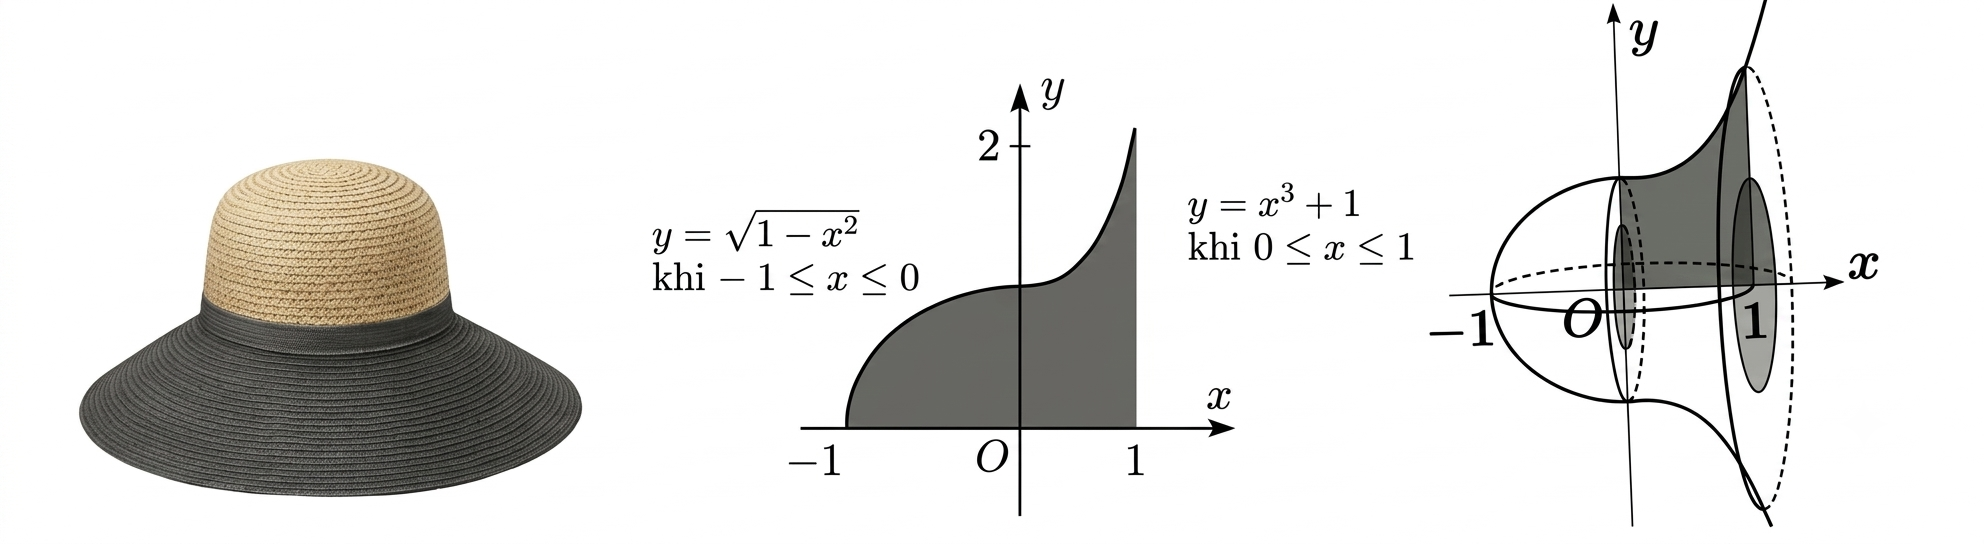
\includegraphics[width=0.7\textwidth]{images/Cau16.png}
\end{figure}
}{
    \textbf{a)} & Diện tích của thiết diện tạo bởi mặt tròn xoay khi cắt mặt phẳng vuông góc với trục \(Ox\) tại \(x = 0\) bằng \(\pi\) (dm\(^2\)).
    & \textcolor{amberorange}{$\bigcirc$} & \textcolor{amberorange}{$\bigcirc$} \\ \hline
    
    \textbf{b)} & Giá trị của hàm số \(f(x)\) khi \(x = 0\) bằng 2.
    & \textcolor{amberorange}{$\bigcirc$} & \textcolor{amberorange}{$\bigcirc$} \\ \hline
    
    \textbf{c)} & Diện tích của hình phẳng \((H)\) là \(S \approx 3,57\) (dm\(^2\)).
    & \textcolor{amberorange}{$\bigcirc$} & \textcolor{amberorange}{$\bigcirc$} \\ \hline
    
    \textbf{d)} & Thể tích của khối tròn xoay trên là \(V \approx 7,26\) (dm\(^3\)).
    & \textcolor{amberorange}{$\bigcirc$} & \textcolor{amberorange}{$\bigcirc$} \\
}

\textit{\textbf{Phần III: Thí sinh trả lời từ câu 17 đến câu 22.}}

\vspace{0.3cm}

% --- CÂU 17 ---
\questionShortAnswer{0}{17}{Một cơ sở sản xuất thiết bị cứu hộ chế tạo một chiếc phao cứu sinh như hình minh họa. Khi đó, theo mặt cắt qua tâm, người ta thấy, bán kính ngoài của phao bằng 35 cm, bán kính trong của phao bằng 25 cm. Phao được làm từ một loại vật liệu đồng chất, có khối lượng riêng bằng \(0,05\) g/cm\(^3\) (coi phao là khối đặc, không có khoảng rỗng bên trong). Tính khối lượng của chiếc phao (đơn vị kg), biết kết quả làm tròn đến hàng phần trăm, số \(\pi\) nhận giá trị bằng \(3,1416\).
\begin{figure}[H]
    \centering
    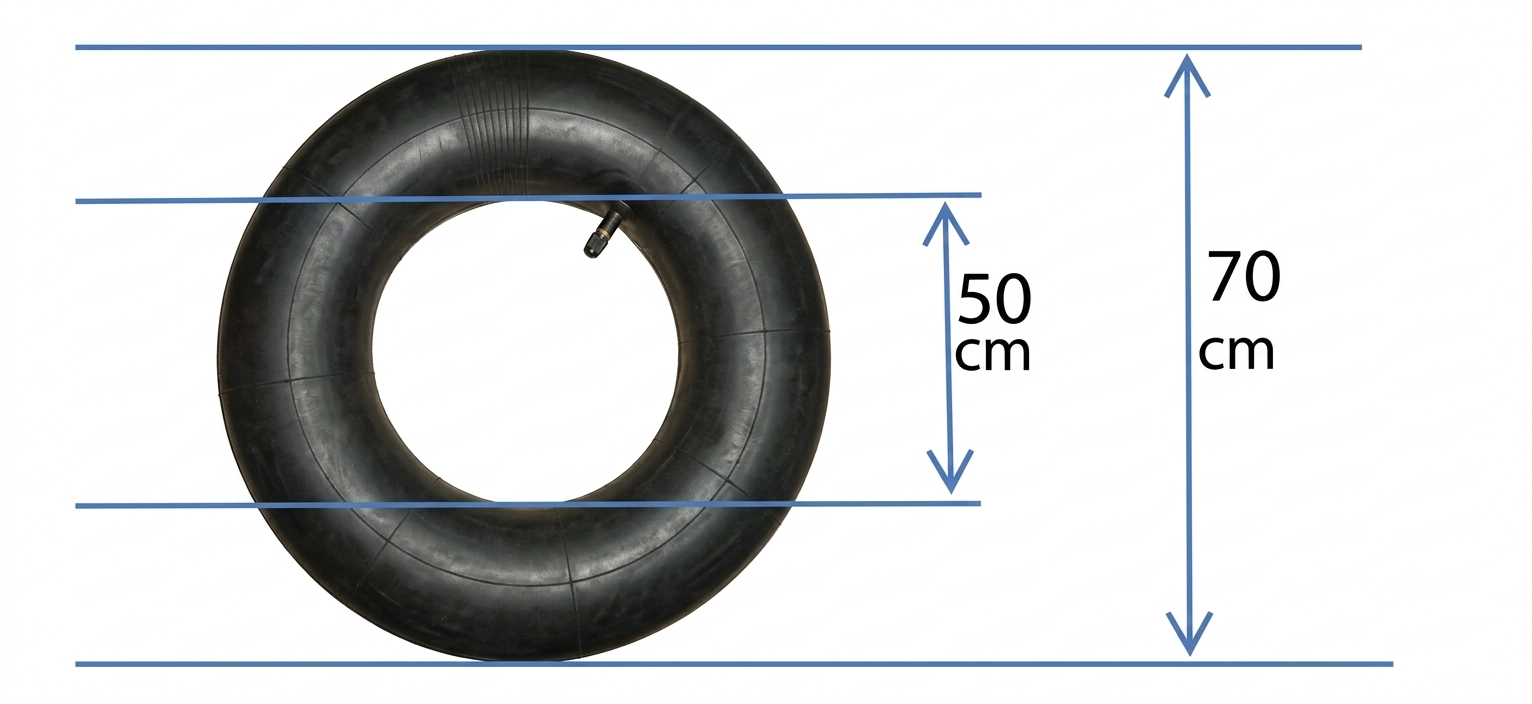
\includegraphics[width=0.7\textwidth]{images/Cau17.png}
\end{figure}
}

% --- CÂU 18 ---
\questionShortAnswer{0}{18}{Một nhà thiết kế dự định thiết kế một logo cho một công ty (xem hình minh họa bên). Đường viền của logo bao gồm nửa đường tròn đường kính \(BC\) bằng 4 cm, hai cung \(AB\) và \(AC\) lần lượt là một phần của các parabol đỉnh \(B\) và đỉnh \(C\), trục đối xứng của mỗi parabol vuông góc với đường thẳng \(BC\). Tính diện tích logo đó, biết tam giác \(ABC\) là tam giác vuông cân tại \(A\) ( làm tròn kết quả đến hàng phần trăm).

\begin{center}
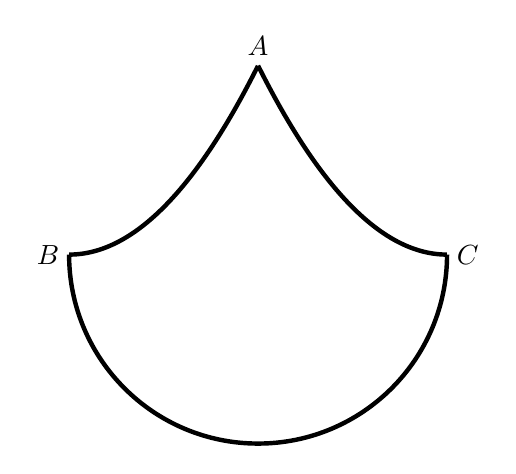
\begin{tikzpicture}[scale=1.2]
    % Định nghĩa tọa độ B, C và A (tam giác ABC vuông cân tại A)
    % Chọn B(-2, 0), C(2, 0) => BC = 4. Điểm A(0, 2)
    \coordinate (B) at (-2, 0);
    \coordinate (C) at (2, 0);
    \coordinate (A) at (0, 2);

    % Vẽ nửa đường tròn đường kính BC ở phía dưới (từ B đến C)
    % Bán kính R = 2, tâm tại (0,0), vẽ cung từ 180 độ đến 360 độ (hoặc 0 độ)
    \draw[ultra thick] (2,0) arc (0:-180:2);

    % Cung AB thuộc parabol đỉnh B(-2, 0) đi qua A(0, 2)
    % Phương trình parabol: y = 0.5 * (x + 2)^2
    \draw[ultra thick, domain=-2:0, samples=100] plot (\x, {0.5*(\x+2)^2});

    % Cung AC thuộc parabol đỉnh C(2, 0) đi qua A(0, 2)
    % Phương trình parabol: y = 0.5 * (x - 2)^2
    \draw[ultra thick, domain=0:2, samples=100] plot (\x, {0.5*(\x-2)^2});

    % Đặt nhãn cho các điểm
    \node[above] at (A) {$A$};
    \node[left] at (B) {$B$};
    \node[right] at (C) {$C$};

\end{tikzpicture}
\end{center}
}

% --- CÂU 19 ---
\questionShortAnswer{0}{19}{Nhiệt độ trung bình của Trái Đất có xu hướng tăng do sự gia tăng nồng độ \(CO_2\) trong khí quyển. Giả sử nồng độ \(CO_2\) trong khí quyển (tính bằng ppm - parts per million) được mô tả bởi hàm số \(C(t) = 420 + 2,5t + 0,02t^2\), trong đó \(t\) được tính theo năm và \(t = 0\) ứng với năm 2025. Mối quan hệ giữa độ tăng nhiệt độ trung bình toàn cầu \(T(t)\) (đơn vị: \(^\circ C\)) và nồng độ \(CO_2\) được mô tả như sau: \(T(t) = \displaystyle\int_{0}^{t} kC(x)dx\) với \(k\) là hằng số. Nếu không có biện pháp giảm phát thải \(CO_2\) và giả sử nhiệt độ trung bình của Trái Đất tăng thêm \(0,99^\circ C\) từ năm 2025 đến năm 2040 thì nhiệt độ trung bình của Trái Đất tăng thêm bao nhiêu \(^\circ C\) từ năm 2025 đến năm 2060? (làm tròn kết quả đến hàng phần trăm).
}

% --- CÂU 20 ---
\questionShortAnswer{0}{20}{Sân vận động Sport Hub – Singapore là sân vận động có mái vòm được chọn để tổ chức lễ bế mạc đại hội thể thao Đông Nam Á năm 2015. Nền sân phẳng là một hình elip (E) có độ dài trục lớn 150 mét và trục bé 90 mét. Một mặt phẳng vuông góc với trục lớn của (E) sẽ cắt elip tại hai điểm A, B và cắt phần dưới của mái vòm theo một cung tròn của đường tròn tâm I thỏa mãn góc \(\widehat{AIB} = 90^\circ\) (Tham khảo hình bên dưới). Các kĩ sư cần tính toán để lắp điều hòa cho sân vận động, mỗi máy điều hòa có công suất 100000 BTU đáp ứng được không gian \(500 m^3\). Hỏi các kĩ sư cần dùng tối thiểu bao nhiêu máy điều hòa để đáp ứng đủ theo yêu cầu kĩ thuật cho sân vận động?
\begin{figure}[H]
    \centering
    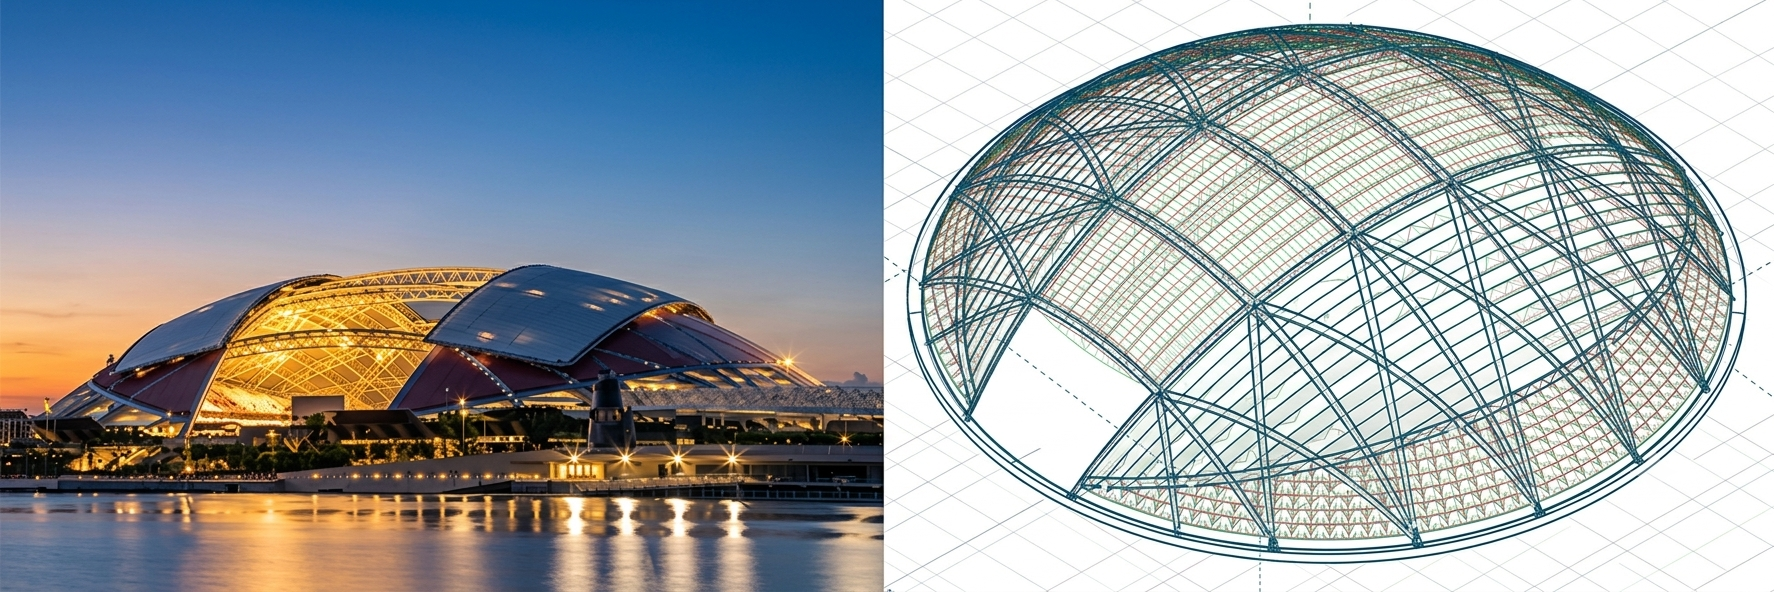
\includegraphics[width=0.7\textwidth]{images/Cau20.1.png}
\end{figure}
\begin{figure}[H]
    \centering
    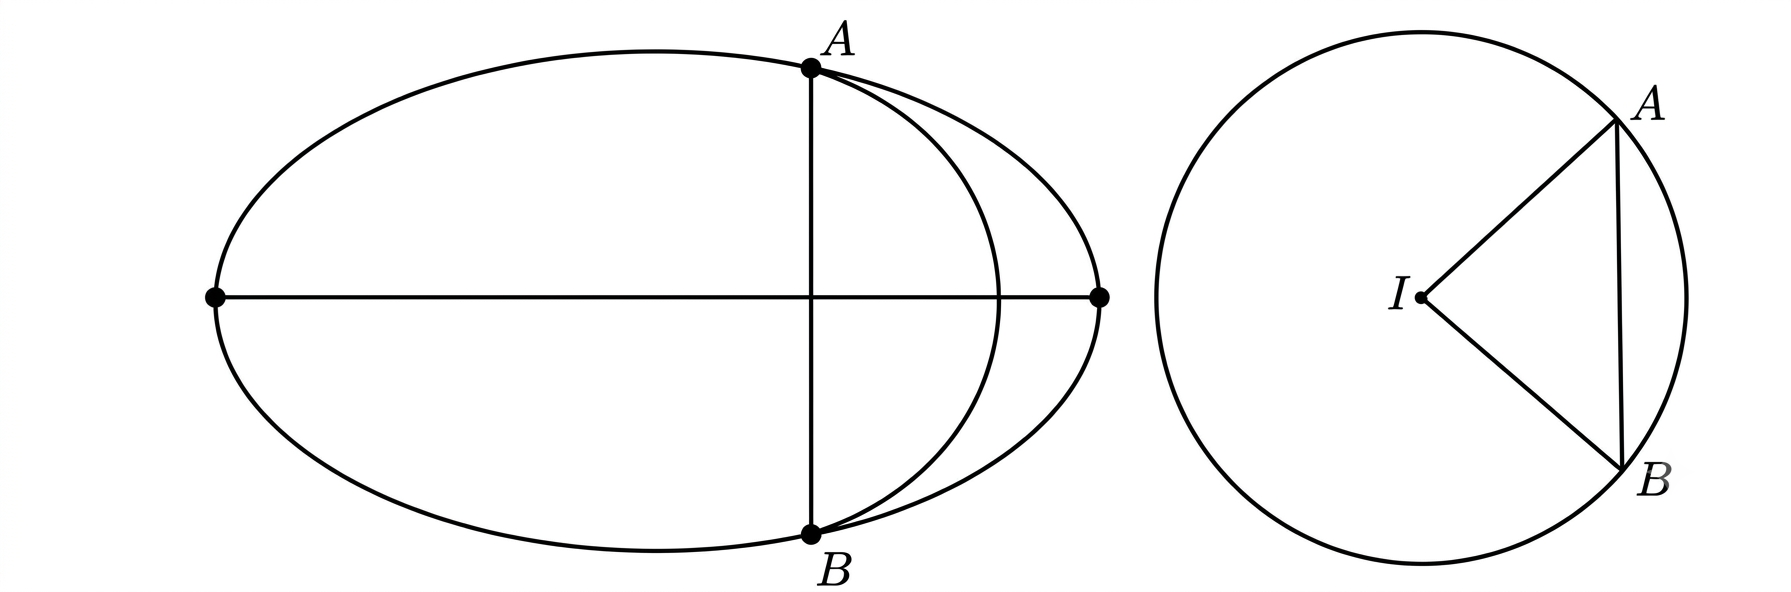
\includegraphics[width=0.7\textwidth]{images/Cau20.2.png}
\end{figure}

}

% --- CÂU 21 ---
\questionShortAnswer{0}{21}{Một vật bắt đầu chuyển động thẳng đều với vận tốc \(v_0 = a\) (m/s) với \(a > 0\). Sau 6 giây chuyển động thì gặp chướng ngại vật nên bắt đầu giảm tốc độ với vận tốc \(v(t) = -\dfrac{5}{2}t + b\) (m/s), (\(t \geq 6\)) cho đến khi dừng hẳn. Biết rằng, kể từ lúc chuyển động đến lúc dừng thì vật đi được quãng đường là 80 (m). Giá trị của \(a^2 - b^2\) bằng bao nhiêu?
}

% --- CÂU 22 ---
\questionShortAnswer{0}{22}{Trong một chương trình giao lưu âm nhạc đón tết vui xuân, ban đầu với sự tham dự của 2100 khán giả. Ban tổ chức đã thống kê số lượng khán giả ở lại sân khấu xem âm nhạc theo thời gian, được mô tả bởi một hàm số liên tục theo \(t \in [0; +\infty)\):
\[
f'(t) = \begin{cases}
2100 - 400t, & 0 \leq t \leq 3 \\
a(t-3)^2 + b, & t > 3
\end{cases}
\]
(trong đó \(f'(t)\) là số khán giả, \(t\) là số giờ kể từ khi chương trình bắt đầu, \(a, b\) là tham số thực), với hàm số \(f(t)\) mô tả tổng sự hiện diện của khán giả theo thời gian \(t\). Sau 3 giờ 30 phút số lượng khán giả ở lại sân khấu là 875. Hỏi từ khi bắt đầu cho đến khi khán giả ra về hết, trung bình mỗi giờ còn bao nhiêu khán giả ở lại tham gia chương trình âm nhạc?
}
\end{document}


%Phần II: Câu 13:ĐSĐS, Câu 14: DDDS, Câu 15: DSSS, Câu 16: DSSD
%Phần III: Câu 17: 0.74, Câu 18: 8.95, Câu 19 2.48, Câu 20: 232, Câu 21: -525, Câu 22: 1050